\documentclass[12pt]{article}
\usepackage[colorlinks=true, linkcolor=blue, breaklinks=true]{hyperref} 
\usepackage{graphicx}
\usepackage{charter,amsmath,amssymb,breakurl}
\usepackage{eulervm}
\usepackage[letterpaper,margin=1in]{geometry}
\usepackage{multicol}
\everymath{\displaystyle}
\author{}\date{Due in class Friday 13 February}
\title{Math 104 Written Assignment 3}\author{}
\begin{document}
\maketitle
\pagestyle{empty}

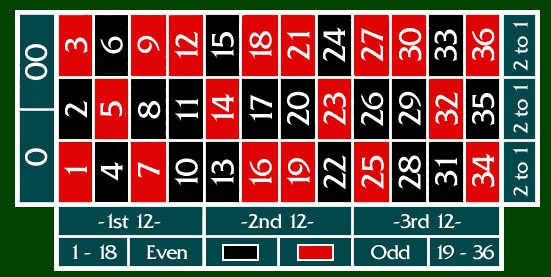
\includegraphics[scale=.5]{RouletteLayout}
\begin{enumerate}
\item A {\em corner} is a roulette bet for any four numbers forming
a contiguous rectangle on the roulette layout, shown above.
For example, a player could make a corner bet on the numbers
$\left\{1,2,4,5\right\}$
\begin{enumerate}
\item Using the formula $\frac{36}{n}-1$ calculate the amount
the casino pays for a $\$1$ corner bet.
\item Calcaulte the probabilities of winning and losing a corner bet.
\item Calculate the expectation for a corner bet.
\end{enumerate}
\end{enumerate}
\end{document}
